%%%%%%%%%%%%%%%%%%%%%%%%%%%%%%%%%%%%%%%%%%%%%%%%%%%%%%%%%%%
%                                                         %
%       This is documentation for the IPK project.        %
%                                                         %
%%%%%%%%%%%%%%%%%%%%%%%%%%%%%%%%%%%%%%%%%%%%%%%%%%%%%%%%%%%


%------------------------------------------------%
%	    CONFIGURATION + IMPORTED PACKAGES        %
%------------------------------------------------%
\documentclass[10pt,a4paper,titlepage]{article}
\usepackage[english]{babel}
\usepackage[utf8]{inputenc}
\usepackage[margin=100pt]{geometry}


\usepackage{graphicx}   % Import pictures
\usepackage{ragged2e}   % fullfill paragraphs
\usepackage{multicol}
\usepackage{lscape}

\newenvironment{changemargin}[2]{%
\begin{list}{}{%
\setlength{\topsep}{0pt}%
\setlength{\leftmargin}{#1}%
\setlength{\rightmargin}{#2}%
\setlength{\listparindent}{\parindent}%
\setlength{\itemindent}{\parindent}%
\setlength{\parsep}{\parskip}%
}%
\item[]}{\end{list}}

\begin{document}
%-----------------------------------------%
%	            TITLE PAGE                %
%-----------------------------------------%
\begin{titlepage}

\begin{center}
% Headings
\textsc{\LARGE Brno University of technology}\\[0.5cm]
\textsc{\large Faculty of Information Technology}\\[8cm]

% Title - lines
{ \huge \bfseries IPK project 1}\\[0.3cm]
{ \Large \bfseries documentation}\\[0.5cm]
{ \bfseries Martin Benes}\\

\end{center}

\end{titlepage}
\newpage

%-----------------------------------------%
%	              DOCUMENT                  %
%-----------------------------------------%

\setcounter{page}{1}
\pagenumbering{arabic}

\section{IPK project documentation}
The task was to create an client-server application in C/C++, that communicates
using BSD sockets and transfers files.

We ought to design our own protocol, that we use for the communication, and
describe it in documentation in detail.

\subsection{Solution}
I started with an analysis of BSD socket interface. Since it has semantics
as C, saving socket into buffer without being possible to reallocate the buffer,
I tried to deal with that in my design, so I would be able to save data using
single function call into rightly sized buffer.


\begin{multicols}{2}
The protocol is described and implemented on two levels of abstraction,
the lower one is encapsulated in class hierarchy and instatiated. It
consists of abstract class {\it Socket}, and inherited {\it ClientSocket}
and {\it ServerSocket}. They also covers the BDS socket interface calling,
so basically only these classes is directly dependent on BSD socket interface.

It enables sending and receiving byte, or string. Sending a variably-sized
data (strings) is preceded with sending a fixed-sized ({\it size\_t})
size of the data. That enables receiver to allocate a buffer of right size,
so the data fits in.

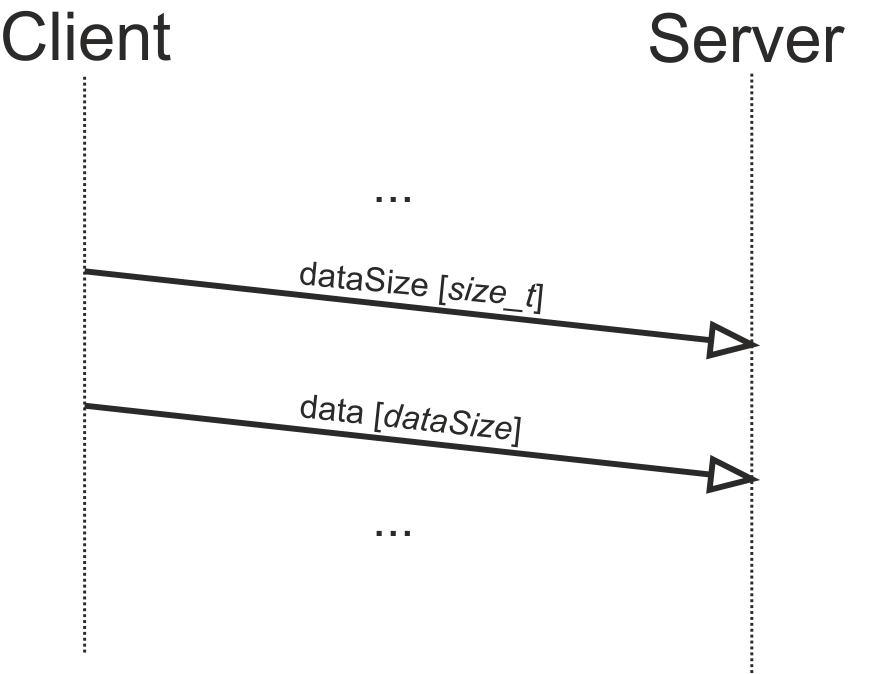
\includegraphics[width=0.55\textwidth]{send_data.png}
\end{multicols}


\begin{multicols}{2}
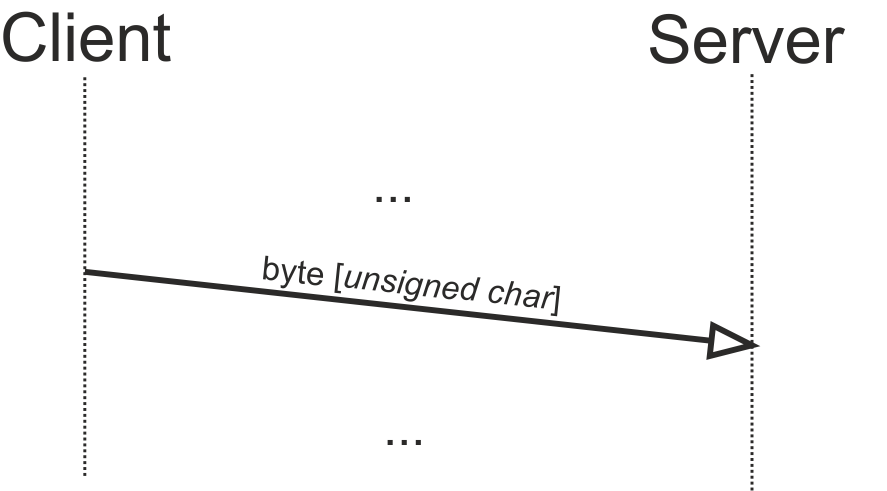
\includegraphics[width=0.4\textwidth]{send_byte.png}

The Socket class and its specializations may send a single byte too.
It is used to send a indication to the opposite side. The client sends
a meta-information, whether it will read or write to the server.

In this case, the sent data is fixed-sized ({\it unsigned~char}),
so it does not have to do the same routine as the above mentioned.
\end{multicols}

The higher abstraction layer (the program itself) uses the services
of the lower. For simplification, the size sending will not
be displayed in images, but I will mention that.

The server is listening on the port and the client is connecting
to the server with explicitly given address and port. The mode
of usage (read/write) is also given.


\begin{multicols}{2}
The read is initiated, when argument {\it -r} is given, following with
a {\it path}. The first to send as a client is a byte 0xFF, that means
the reading mode is selected.

The second thing to send is the {\it full path of file}. Afterwards, the {\it file}
itself is expected to receive from the server in the form of string.

The semantics of sending a string are used here, as same as while sending
a file path.

When the file data arrives, they are written into the file of the same name,
as the received one.

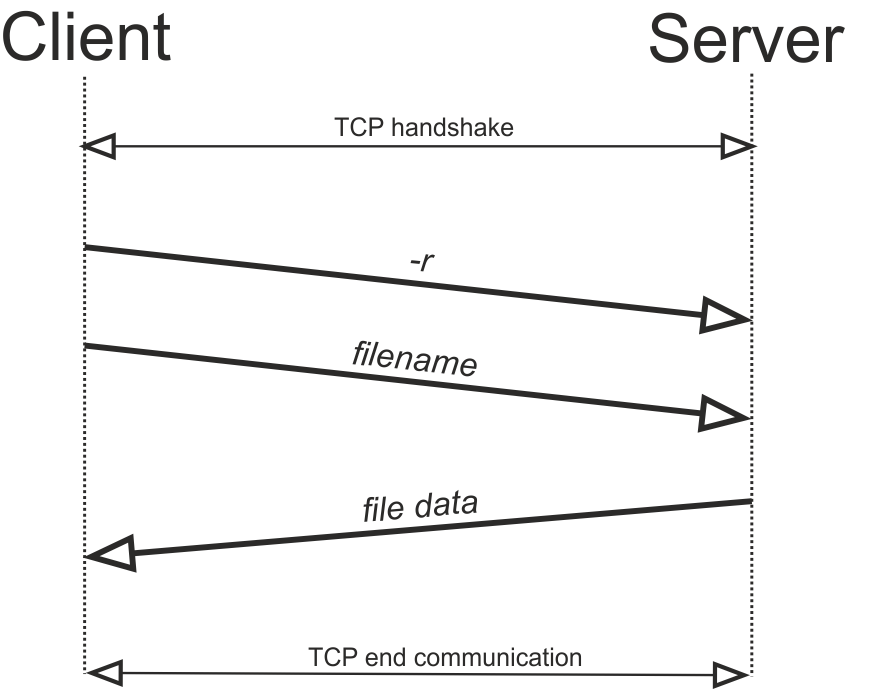
\includegraphics[width=0.5\textwidth]{read.png}
\end{multicols}


\begin{multicols}{2}
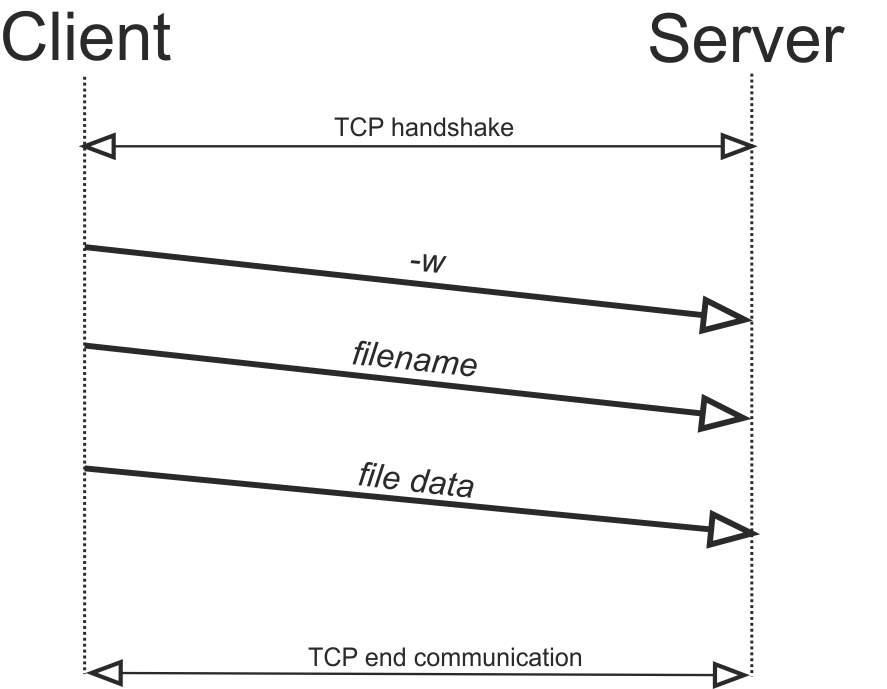
\includegraphics[width=0.5\textwidth]{write.png}

The write is similar as read with slight differences, it is initialized
with given argument {\it -w} and {\it path} afterwards. The first byte
is 0x00, indicating write mode.

Then the client sends {\it the name of the file} (without the path), on the
server, it will be located in the working directory.

The client follows with sending {\it the file data}. Again, it is done
with the mentioned method of sending variably-sized strings.

The server then writes the received data to the file.

\end{multicols}


\end{document}
